\documentclass[12pt, english, reqno, oneside]{smfart}
\usepackage[utf8]{inputenc}
\usepackage{amsmath,amssymb,amsthm,bm,mathtools}
\usepackage[colorlinks=true,
            linkcolor=blue,
            filecolor=blue,
            citecolor=red,
            urlcolor=blue, 
            colorlinks=true]{hyperref}
\usepackage{tikz}
\usepackage{tikz-cd}
\usetikzlibrary{arrows}
\usetikzlibrary{decorations.pathmorphing}
\usetikzlibrary{decorations.markings}
\usetikzlibrary{arrows.meta,bending}
\usetikzlibrary{decorations.pathreplacing,calligraphy}
\usetikzlibrary{shapes.geometric}
\usetikzlibrary{patterns}

\begin{document}

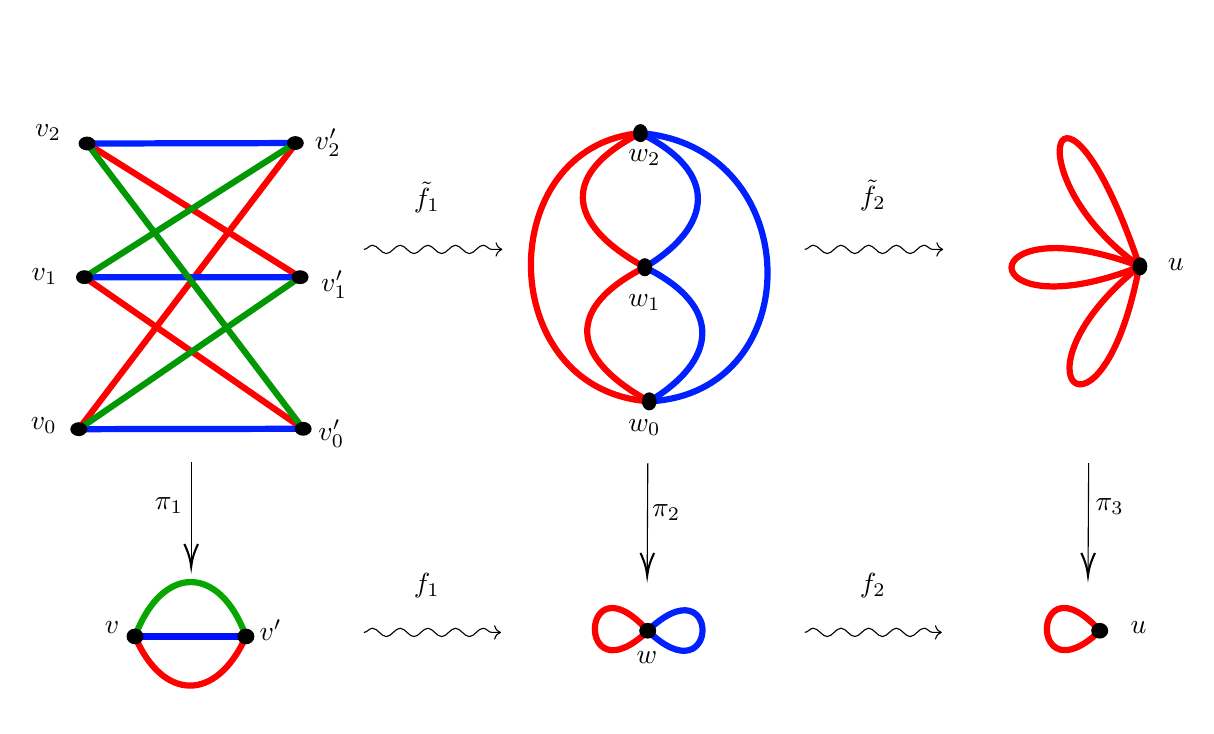
\begin{tikzpicture}[x=0.75pt,y=0.75pt,yscale=-1,xscale=1]

\draw [color={rgb, 255:red, 8; green, 167; blue, 0 }  ,draw opacity=1 ][line width=2.25]    (61.61,326.32) .. controls (74.87,291.12) and (102.62,291.66) .. (115.06,326.32) ;
\draw [color={rgb, 255:red, 255; green, 0; blue, 0 }  ,draw opacity=1 ][line width=2.25]    (61.61,326.32) .. controls (74.87,357.43) and (100.71,358.35) .. (115.06,326.32) ;
\draw [color={rgb, 255:red, 0; green, 13; blue, 255 }  ,draw opacity=1 ][line width=2.25]    (61.61,326.32) -- (115.06,326.32) ;

\draw [color={rgb, 255:red, 255; green, 0; blue, 0 }  ,draw opacity=1 ][line width=2.25]    (38.5,88.83) -- (141.17,153.23) ;
\draw [color={rgb, 255:red, 255; green, 0; blue, 0 }  ,draw opacity=1 ][line width=2.25]    (37.25,153.22) -- (142.64,226.28) ;
\draw [color={rgb, 255:red, 255; green, 0; blue, 0 }  ,draw opacity=1 ][line width=2.25]    (34.51,226.46) -- (139.7,88.05) ;
\draw [color={rgb, 255:red, 0; green, 32; blue, 255 }  ,draw opacity=1 ][line width=2.25]    (38.5,88.83) -- (138.87,88.61) ;
\draw [color={rgb, 255:red, 0; green, 32; blue, 255 }  ,draw opacity=1 ][line width=2.25]    (34.51,226.46) -- (142.64,226.28) ;
\draw [color={rgb, 255:red, 0; green, 32; blue, 255 }  ,draw opacity=1 ][line width=2.25]    (37.25,153.22) -- (141.17,153.23) ;
\draw [color={rgb, 255:red, 1; green, 152; blue, 4 }  ,draw opacity=1 ][line width=2.25]    (37.25,153.22) -- (139.7,88.05) ;
\draw [color={rgb, 255:red, 1; green, 152; blue, 4 }  ,draw opacity=1 ][line width=2.25]    (38.5,88.83) -- (142.64,226.28) ;
\draw [color={rgb, 255:red, 1; green, 152; blue, 4 }  ,draw opacity=1 ][line width=2.25]    (34.51,226.46) -- (141.17,153.23) ;
\draw  [fill={rgb, 255:red, 0; green, 0; blue, 0 }  ,fill opacity=1 ] (57.8,326.32) .. controls (57.8,324.38) and (59.5,322.8) .. (61.61,322.8) .. controls (63.72,322.8) and (65.42,324.38) .. (65.42,326.32) .. controls (65.42,328.26) and (63.72,329.83) .. (61.61,329.83) .. controls (59.5,329.83) and (57.8,328.26) .. (57.8,326.32) -- cycle ;
\draw  [fill={rgb, 255:red, 0; green, 0; blue, 0 }  ,fill opacity=1 ] (111.25,326.32) .. controls (111.25,324.38) and (112.96,322.81) .. (115.06,322.81) .. controls (117.17,322.81) and (118.87,324.38) .. (118.87,326.32) .. controls (118.87,328.26) and (117.17,329.84) .. (115.06,329.84) .. controls (112.96,329.84) and (111.25,328.26) .. (111.25,326.32) -- cycle ;
\draw  [fill={rgb, 255:red, 0; green, 0; blue, 0 }  ,fill opacity=1 ] (138.85,226.28) .. controls (138.85,224.59) and (140.55,223.22) .. (142.64,223.22) .. controls (144.73,223.22) and (146.43,224.59) .. (146.43,226.28) .. controls (146.43,227.97) and (144.73,229.35) .. (142.64,229.35) .. controls (140.55,229.35) and (138.85,227.97) .. (138.85,226.28) -- cycle ;
\draw  [fill={rgb, 255:red, 0; green, 0; blue, 0 }  ,fill opacity=1 ] (137.38,153.23) .. controls (137.38,151.54) and (139.08,150.17) .. (141.17,150.17) .. controls (143.27,150.17) and (144.96,151.54) .. (144.96,153.23) .. controls (144.96,154.92) and (143.27,156.3) .. (141.17,156.3) .. controls (139.08,156.3) and (137.38,154.92) .. (137.38,153.23) -- cycle ;
\draw  [fill={rgb, 255:red, 0; green, 0; blue, 0 }  ,fill opacity=1 ] (135.08,88.61) .. controls (135.08,86.92) and (136.78,85.55) .. (138.87,85.55) .. controls (140.96,85.55) and (142.66,86.92) .. (142.66,88.61) .. controls (142.66,90.3) and (140.96,91.67) .. (138.87,91.67) .. controls (136.78,91.67) and (135.08,90.3) .. (135.08,88.61) -- cycle ;
\draw  [fill={rgb, 255:red, 0; green, 0; blue, 0 }  ,fill opacity=1 ] (30.72,226.46) .. controls (30.72,224.76) and (32.42,223.39) .. (34.51,223.39) .. controls (36.6,223.39) and (38.3,224.76) .. (38.3,226.46) .. controls (38.3,228.15) and (36.6,229.52) .. (34.51,229.52) .. controls (32.42,229.52) and (30.72,228.15) .. (30.72,226.46) -- cycle ;
\draw  [fill={rgb, 255:red, 0; green, 0; blue, 0 }  ,fill opacity=1 ] (33.46,153.22) .. controls (33.46,151.52) and (35.16,150.15) .. (37.25,150.15) .. controls (39.35,150.15) and (41.04,151.52) .. (41.04,153.22) .. controls (41.04,154.91) and (39.35,156.28) .. (37.25,156.28) .. controls (35.16,156.28) and (33.46,154.91) .. (33.46,153.22) -- cycle ;
\draw  [fill={rgb, 255:red, 0; green, 0; blue, 0 }  ,fill opacity=1 ] (34.71,88.83) .. controls (34.71,87.13) and (36.41,85.76) .. (38.5,85.76) .. controls (40.59,85.76) and (42.29,87.13) .. (42.29,88.83) .. controls (42.29,90.52) and (40.59,91.89) .. (38.5,91.89) .. controls (36.41,91.89) and (34.71,90.52) .. (34.71,88.83) -- cycle ;
\draw    (88.68,242.38) -- (88.68,290.73) ;
\draw [shift={(88.68,292.73)}, rotate = 270] [color={rgb, 255:red, 0; green, 0; blue, 0 }  ][line width=0.75]    (10.93,-3.29) .. controls (6.95,-1.4) and (3.31,-0.3) .. (0,0) .. controls (3.31,0.3) and (6.95,1.4) .. (10.93,3.29)   ;
\draw    (308.68,242.84) -- (308.39,295.05) ;
\draw [shift={(308.38,297.05)}, rotate = 270.32] [color={rgb, 255:red, 0; green, 0; blue, 0 }  ][line width=0.75]    (10.93,-3.29) .. controls (6.95,-1.4) and (3.31,-0.3) .. (0,0) .. controls (3.31,0.3) and (6.95,1.4) .. (10.93,3.29)   ;

\path[draw, ->, decorate, decoration ={snake, amplitude = 1.5}] (171.87,139.86) -- (238.62,139.86);    


\path[draw, ->, decorate, decoration ={snake, amplitude = 1.5}] (171.87,324.39) -- (237.93,324.39);    

\draw [color={rgb, 255:red, 255; green, 0; blue, 0 }  ,draw opacity=1 ][line width=2.25]    (308.81,323.59) .. controls (273.62,357.19) and (275.68,286.8) .. (308.64,323.59) ;
\draw [color={rgb, 255:red, 0; green, 32; blue, 255 }  ,draw opacity=1 ][line width=2.25]    (308.58,323.59) .. controls (344.2,289.53) and (343.51,357.19) .. (308.64,323.59) ;
\draw [color={rgb, 255:red, 255; green, 0; blue, 0 }  ,draw opacity=1 ][line width=2.25]    (305.12,83.83) .. controls (267.43,102.96) and (268.12,126.88) .. (307.25,148.45) ;
\draw [color={rgb, 255:red, 255; green, 0; blue, 0 }  ,draw opacity=1 ][line width=2.25]    (307.25,148.45) .. controls (269.56,167.58) and (270.25,191.5) .. (309.37,213.07) ;
\draw [color={rgb, 255:red, 255; green, 0; blue, 0 }  ,draw opacity=1 ][line width=2.25]    (305.12,83.83) .. controls (233.75,90.18) and (234.43,207.73) .. (309.37,213.07) ;
\draw [color={rgb, 255:red, 0; green, 32; blue, 255 }  ,draw opacity=1 ][line width=2.25]    (305.12,83.83) .. controls (385,90.18) and (387.06,209.09) .. (309.37,213.07) ;
\draw [color={rgb, 255:red, 0; green, 32; blue, 255 }  ,draw opacity=1 ][line width=2.25]    (305.12,83.83) .. controls (343.75,102.96) and (339.62,128.93) .. (307.25,148.45) ;
\draw [color={rgb, 255:red, 0; green, 32; blue, 255 }  ,draw opacity=1 ][line width=2.25]    (307.25,148.45) .. controls (345.87,167.58) and (341.75,193.55) .. (309.37,213.07) ;
\draw  [fill={rgb, 255:red, 0; green, 0; blue, 0 }  ,fill opacity=1 ] (301.84,83.83) .. controls (301.84,81.57) and (303.31,79.75) .. (305.12,79.75) .. controls (306.93,79.75) and (308.41,81.57) .. (308.41,83.83) .. controls (308.41,86.08) and (306.93,87.9) .. (305.12,87.9) .. controls (303.31,87.9) and (301.84,86.08) .. (301.84,83.83) -- cycle ;
\draw  [fill={rgb, 255:red, 0; green, 0; blue, 0 }  ,fill opacity=1 ] (303.96,148.45) .. controls (303.96,146.2) and (305.43,144.37) .. (307.25,144.37) .. controls (309.06,144.37) and (310.53,146.2) .. (310.53,148.45) .. controls (310.53,150.7) and (309.06,152.53) .. (307.25,152.53) .. controls (305.43,152.53) and (303.96,150.7) .. (303.96,148.45) -- cycle ;
\draw  [fill={rgb, 255:red, 0; green, 0; blue, 0 }  ,fill opacity=1 ] (306.09,213.07) .. controls (306.09,210.82) and (307.56,208.99) .. (309.37,208.99) .. controls (311.19,208.99) and (312.66,210.82) .. (312.66,213.07) .. controls (312.66,215.32) and (311.19,217.15) .. (309.37,217.15) .. controls (307.56,217.15) and (306.09,215.32) .. (306.09,213.07) -- cycle ;
\draw  [fill={rgb, 255:red, 0; green, 0; blue, 0 }  ,fill opacity=1 ] (304.82,323.59) .. controls (304.82,321.65) and (306.53,320.07) .. (308.64,320.07) .. controls (310.74,320.07) and (312.45,321.65) .. (312.45,323.59) .. controls (312.45,325.53) and (310.74,327.1) .. (308.64,327.1) .. controls (306.53,327.1) and (304.82,325.53) .. (304.82,323.59) -- cycle ;


\draw    (521.08,242.82) -- (520.79,295.03) ;
\draw [shift={(520.77,297.03)}, rotate = 270.32] [color={rgb, 255:red, 0; green, 0; blue, 0 }  ][line width=0.75]    (10.93,-3.29) .. controls (6.95,-1.4) and (3.31,-0.3) .. (0,0) .. controls (3.31,0.3) and (6.95,1.4) .. (10.93,3.29)   ;


\path[draw, ->, decorate, decoration ={snake, amplitude = 1.5}]  (384.26,139.85) -- (451.01,139.85);



\path[draw, ->, decorate, decoration ={snake, amplitude = 1.5}] (384.26,324.37) -- (450.33,324.37);    
\draw [color={rgb, 255:red, 255; green, 0; blue, 0 }  ,draw opacity=1 ][line width=2.25]    (526.58,323.57) .. controls (491.39,357.17) and (493.45,286.78) .. (526.4,323.57) ;
\draw  [fill={rgb, 255:red, 0; green, 0; blue, 0 }  ,fill opacity=1 ] (522.59,323.57) .. controls (522.59,321.63) and (524.3,320.06) .. (526.4,320.06) .. controls (528.51,320.06) and (530.21,321.63) .. (530.21,323.57) .. controls (530.21,325.51) and (528.51,327.08) .. (526.4,327.08) .. controls (524.3,327.08) and (522.59,325.51) .. (522.59,323.57) -- cycle ;
\draw [color={rgb, 255:red, 255; green, 0; blue, 0 }  ,draw opacity=1 ][line width=2.25]    (545.97,148.02) .. controls (463.71,180.87) and (462.81,116.91) .. (545.79,148.02) ;
\draw [color={rgb, 255:red, 255; green, 0; blue, 0 }  ,draw opacity=1 ][line width=2.25]    (545.79,148.02) .. controls (482.87,103.89) and (507.04,34.52) .. (545.62,148.02) ;
\draw [color={rgb, 255:red, 255; green, 0; blue, 0 }  ,draw opacity=1 ][line width=2.25]    (545.62,148.02) .. controls (479.82,200.69) and (527.27,243.94) .. (545.44,148.02) ;
\draw  [fill={rgb, 255:red, 0; green, 0; blue, 0 }  ,fill opacity=1 ] (542.51,148.02) .. controls (542.51,145.77) and (543.98,143.95) .. (545.79,143.95) .. controls (547.61,143.95) and (549.08,145.77) .. (549.08,148.02) .. controls (549.08,150.28) and (547.61,152.1) .. (545.79,152.1) .. controls (543.98,152.1) and (542.51,150.28) .. (542.51,148.02) -- cycle ;

% Text Node
\draw (45.87,317.7) node [anchor=north west][inner sep=0.75pt]    {$v$};
% Text Node
\draw (120.34,317.01) node [anchor=north west][inner sep=0.75pt]    {$v'$};
% Text Node
\draw (148.72,220.7) node [anchor=north west][inner sep=0.75pt]    {$v_{0} '$};
% Text Node
\draw (147,80.4) node [anchor=north west][inner sep=0.75pt]    {$v_{2} '$};
% Text Node
\draw (10.17,219.7) node [anchor=north west][inner sep=0.75pt]    {$v_{0}$};
% Text Node
\draw (10.53,147.67) node [anchor=north west][inner sep=0.75pt]    {$v_{1}$};
% Text Node
\draw (12.26,78.58) node [anchor=north west][inner sep=0.75pt]    {$v_{2}$};
% Text Node
\draw (150.08,149.03) node [anchor=north west][inner sep=0.75pt]    {$v_{1} '$};
% Text Node
\draw (69.9,257.92) node [anchor=north west][inner sep=0.75pt]    {$\pi _{1}$};
% Text Node
\draw (302,332.4) node [anchor=north west][inner sep=0.75pt]    {$w$};
% Text Node
\draw (298,220.4) node [anchor=north west][inner sep=0.75pt]    {$w_{0}$};
% Text Node
\draw (298,90.4) node [anchor=north west][inner sep=0.75pt]    {$w_{2}$};
% Text Node
\draw (298,160.4) node [anchor=north west][inner sep=0.75pt]    {$w_{1}$};
% Text Node
\draw (309.54,261.34) node [anchor=north west][inner sep=0.75pt]    {$\pi _{2}$};
% Text Node
\draw (194.68,105.96) node [anchor=north west][inner sep=0.75pt]    {$\tilde{f}_{1}$};
% Text Node
\draw (194.68,294.79) node [anchor=north west][inner sep=0.75pt]    {$f_{1}$};
% Text Node
\draw (540,318) node [anchor=north west][inner sep=0.75pt]    {$u$};
% Text Node
\draw (523.14,258.76) node [anchor=north west][inner sep=0.75pt]    {$\pi _{3}$};
% Text Node
\draw (409.55,105.06) node [anchor=north west][inner sep=0.75pt]    {$\tilde{f}_{2}$};
% Text Node
\draw (409.55,294.79) node [anchor=north west][inner sep=0.75pt]    {$f_{2}$};
% Text Node
\draw (558,143) node [anchor=north west][inner sep=0.75pt]    {$u$};

\end{tikzpicture}

\end{document}